\documentclass[11pt]{article}
\renewcommand{\rmdefault}{ptm}
\usepackage[scaled=0.92]{helvet}
\usepackage{courier,xcolor,colortbl,listings,parskip,graphicx,fancyvrb,fancyhdr,lastpage}
\usepackage{float,framed}
\normalfont
\usepackage[T1]{fontenc}
\setlength{\parskip}{7pt}
\usepackage[toc,page]{appendix}
\usepackage[hmargin=2.5cm,vmargin=2cm]{geometry}
\usepackage[utf8]{inputenc}
\usepackage[brazil]{babel}
\pagestyle{fancy}
\setlength{\headheight}{120pt}
\setlength{\headsep}{30pt}
\setlength{\textheight}{550pt}
\renewcommand{\headrulewidth}{0pt}
\lhead{}
\rhead{}
\chead{
\includegraphics{brasao.jpg}\\
        \large \textbf{PRESIDÊNCIA DA REPÚBLICA}\\
        \large SECRETARIA-GERAL\\
        \large Secretaria-Executiva}
\cfoot{}
\rfoot{\thepage /\pageref{LastPage}}
\hyphenation{par-ti-ci-pa-ção}
\bibliographystyle{ieeetr}

\newcommand{\MyName}{Daniela Soares Feitosa}
\newcommand{\MyEmail}{daniela@colivre.coop.br}
\newcommand{\ContractNumber}{2013/xxxxxx}
\newcommand{\ProjectCode}{Projeto PNUD BRA/12/018}
\newcommand{\NomeSecretaria}{Secretaria Geral da Presidência da República}
\newcommand{\SiglaSecretaria}{SG/PR}
\newcommand{\ProductNumber}{04}
\newcommand{\ProductDescription}{Documento com proposta para
desenvolvimento do código do aplicativo de consulta pública, do código
de integração dele com o portal e do painel de controle e administração,
contendo exemplos e códigos.}
\newcommand{\MesEntrega}{Setembro de 2013}
\newcommand{\DiaEntrega}{05}

\begin{document}
\lstset{language=Ruby}
\definecolor{light-gray}{gray}{0.95}
\lstdefinestyle{codeFrame}{backgroundcolor=\color{light-gray},frame=lines}

\textbf{\ProjectCode \ -} \ProductDescription

\vspace{3cm}

\begin{minipage}{0.5\textwidth}
  \textbf{Consultora: \MyName}
  \newline
  \textbf{Contrato nº: \ContractNumber}
  \newline
  \textbf{Produto / nº: \ProductNumber}
\end{minipage}

\vspace{2cm}

\textbf{Assinatura do Consultor}

\begin{framed}
Local e data: Brasília/DF, \line(1,0){20} \ de \line(1,0){100} \ de 2014
\newline
\newline
Assinatura do Consultor: \line(1,0){300}
\end{framed}

\vspace{1cm}

\textbf{Assinatura do Supervisor}

\begin{framed}
Atesto que os serviços foram prestados conforme estabelecido no Contrato
de Consultoria.
\newline
\newline
Local e data: Brasília/DF, \line(1,0){20} \ de \line(1,0){100} \ de 2014
\newline
\newline
Assinatura e Carimbo: \line(1,0){300}
\end{framed}

\clearpage
\newcolumntype{g}{>{\columncolor{light-gray}}l}

\begin{center}
  \begin{tabular}{| g | p{10cm} |}
    \hline
    \textbf{Título} & \ProductDescription \\ \hline
    \textbf{Língua do documento} & Português - Brasil \\ \hline
    \textbf{Documentação de referência} & Português \\ \hline
    \textbf{Unidade responsável} & \NomeSecretaria \
(\SiglaSecretaria) \\ \hline
    \textbf{Criador} & \MyName - \MyEmail \\ \hline
    \textbf{Taxonomias} & Desenvolvimento \\ \hline
    \textbf{Data de aprovação} & mês de ano \\ \hline
    \textbf{Público} & \SiglaSecretaria, Parceiros e Sociedade
Civil \\ \hline
    \textbf{Aplicabilidade} & Explicar isso aqui \\ \hline
    \textbf{Faz parte do} & \ProjectCode \\ \hline
    \textbf{Em conformidade com a} & \NomeSecretaria \\ \hline
    \textbf{Documentos anexos} & Nenhum \\ \hline
    \textbf{Revisado em} & dia mês ano \\ \hline
  \end{tabular}
\end{center}

\clearpage

\tableofcontents
\clearpage
\listoffigures

\clearpage

\section{Apresentação}

Em consonância com os objetivos e cronograma previsto no âmbito do
projeto BRA/12/018:
\textbf{Desenvolvimento de Metodologias de Articulação e Gestão de
Políticas Públicas para Promoção da Democracia Participativa},
firmado entre a Secretaria-Geral da Presidência da República
(SG/PR) e o Programa das Nações Unidas para o Desenvolvimento (PNUD),
o presente documento apresenta a proposta para
desenvonlvimento do código do aplicativo de consulta pública, do código
de integração dele com o portal e do painel de controle e
administração, contendo exemplos e códigos.

Essa proposta está configurada como produto 4 da consultoria técnica
para especificação da construção dos códigos das metodologias de
organização da informação e interação participativa do portal de
participação social.

Neste documento será apresentada a especificação e
modelagem do código para auxiliar os órgãos e entidades do
Governo Federal no relacionamento e articulação com os movimentos
sociais através do Portal de Consulta Pública, um dos canais que
possibilita a consulta e participação popular na discussão e na definição
da agenda prioritária do país.

Como o Portal de Consulta Pública utiliza o software livre Noosfero,
plataforma web para redes sociais, o código produzido deverá ser público
e divulgado para a comunidade e para os que desenvolvem e se utilizam do
software.

O código foi desenvolvido para ser utilizado como um plugin do Noosfero.
O plugin de Classificação de Comentários ( {\it CommentClassification} )
permite:

\begin{itemize}
  \item Gestão de {\it Etiquetas} e {\it Status} dos comentários;
  \item Habilitação da funcionalidade de Apoio ({\it Support}) à
comentários;
    \subitem Visualização da listagem de usuários que apoiam um comentário;
  \item Possibilidade de definir uma Etiqueta a um comentário;
  \item Possibilidade de adicionar {\it Status} e justificativas a um
comentário;
    \subitem Possibilidade de concordar com uma justificativa;
  \item Possibilidade de sugerir novas redações aos trechos disponíveis
na consulta pública;
  \item Gestão das possibilidades de classificação dos comentários por
perfil;
  \item Visualização das estatísticas das classificações;
  \item Exportação em CSV dos trechos, comentários, etiquetas, status,
justificativas e novas redações;
\end{itemize}

Como conteúdo deste documento também serão apresentados as telas
iniciais para interação com o plugin, incluindo instruções passo a
passo para a utilização do Portal de Consulta Pública tanto para usuário
visitante como administrador do ambiente.

\section{Plugin de Classificação de Comentários}

O Plugin de Classificação de Comentários permite algumas formas de
classificar um comentário: etiquetas, status e suporte.

O plugin foi desenvolvido para ser utilizado no Noosfero e pode ser
habilitado e desabilitado em qualquer instalação do Noosfero.

O código do plugin pode ser visto no Apêndice~\ref{App:PluginCode}

Para disponibilizar um plugin num ambiente do Noosfero, é necessário
primeiro habilitá-lo no servidor:

\begin{verbatim}

$ ./script/noosfero-plugins enable comment_classification

\end{verbatim}

E depois habilitar no ambiente. A tela de administração de plugins está
sendo mostrada na Figura~\ref{fig:environment-admin-page}.

\begin{figure}[h]
\center
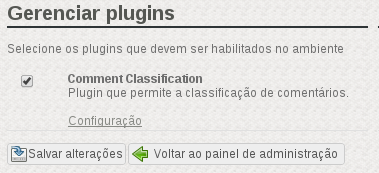
\includegraphics[scale=0.6]{environment-admin-page.png}
\caption{Tela de administração dos plugins num ambiente Noosfero}
\label{fig:environment-admin-page}
\end{figure}

Abaixo da descrição do plugin o administrador do ambiente poderá
gerenciar as classificações, clicando no link Configuração que pode ser
visto na Figura~\ref{fig:environment-admin-page}. A tela representada na
Figura~\ref{fig:plugin-admin-page} mostra os links de administração das
Etiquetas e Status.

\begin{figure}[h]
\center
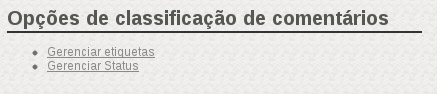
\includegraphics[scale=0.6]{plugin-admin-page.png}
\caption{Tela de administração do plugin}
\label{fig:plugin-admin-page}
\end{figure}

\section{Etiquetas}

As etiquetas permitem a classificação única dos comentários.

\subsection{Definição}

Foi definida uma nova classe {\it Label}
(Apêndice~\ref{App:PluginLabel}) no Plugin de classificação de
comentários para a inclusão da funcionalidade de Classificação por
Etiquetas. Cada comentário pode ser classificado por uma Etiqueta, que possui os
seguintes atributos:
\begin{itemize}
  \item Nome ({\it name}): cada etiqueta terá um nome único, que a representará no
ambiente;
  \item Cor ({\it color}): será utilizada ao mostrar a etiqueta de um comentário. As
cores permitem que uma informação seja absorvida pelo leitor de forma
mais rápida, então a escolha das cores deve ter alguma relação com a
ideia que a Etiqueta deve passar;
  \item Habilitado ({\it enabled}): As etiquetas podem ser habilitadas e desabilitadas
pelos administradores. Apenas as etiquetas habilitadas estarão
disponíveis para classificação dos comentários;
  \item Dono ({\it owner}): Relaciona a etiqueta com o tipo que a criou.
As etiquetas podem ser definidas no ambiente e
nos perfis. As etiquetas definidas no contexto do ambiente ficarão
disponíveis para todos os perfis da rede e as definidas no contexto do
perfil ficarão disponíveis apenas para os perfis.
\end{itemize}

O sistema registra quando um usuário adiciona uma Etiqueta a um
comentário. A classe apresentada no
Apêndice~\ref{App:PluginCommentLabelUser} mostra as relações e
validações da relação. Quando um usuário classifica um comentário é
criada a relação no banco de dados com os seguintes atributos:
\begin{itemize}
  \item Profile ({\it profile}): Referencia o perfil que definiu a
etiqueta;
  \item Comment ({\it comment}): Referencia o comentário classificado;
  \item Label ({\it label}): Referencia a etiqueta definida;
\end{itemize}

As definições dessas classes e seus atributos podem ser vistas na
Figura~\ref{fig:labels-model}.

\begin{figure}[h]
\center
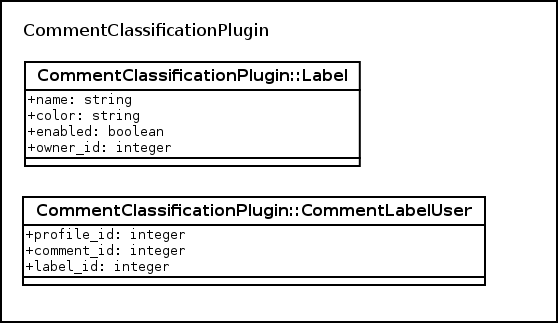
\includegraphics[scale=0.5]{labels-model.png}
\caption{Modelagem das classes para definir uma etiqueta a um comentário}
\label{fig:labels-model}
\end{figure}

O próprio proponente do comentário pode classificar inicialmente o
comentário e o avaliador pode alterar a classificação do proponente. Os
avaliadores são usuários do ambiente com perfil de moderação de
comentários no perfil.

\subsection{Administração}

Para a gestão de {\it Etiquetas} dos comentários foi criada uma tela com
a listagem das etiquetas disponíveis no ambiente
(Figura~\ref{fig:plugin-label-admin}). Nessa página o administrador
do ambiente poderá criar, editar e remover qualquer uma das etiquetas
listadas.

\begin{figure}[h]
\center
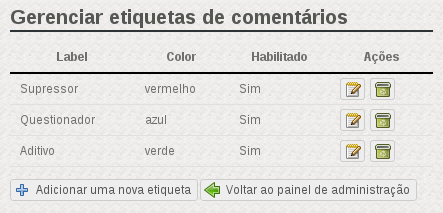
\includegraphics[scale=0.5]{plugin-label-admin.png}
\caption{Tela de gestão das Etiquetas}
\label{fig:plugin-label-admin}
\end{figure}

O formulário de criação de Etiquetas pode ser visto na
Figura~\ref{fig:new-label-page}. Nessa página o administrador
do ambiente poderá definir os atributos da etiqueta.

\begin{figure}[h]
\center
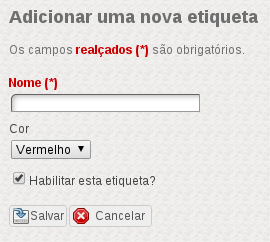
\includegraphics[scale=0.5]{new-label-page.png}
\caption{Criação de etiquetas}
\label{fig:new-label-page}
\end{figure}


\subsection{Utilização}

No formulário de criação de comentários do Noosfero foi adicionado um
campo extra que permite que um usuário escolha uma Etiqueta para
classificar seu comentário (Figura~\ref{fig:comment-add}).

Cada comentário poderá ter apenas uma etiqueta. As etiquetas serão
utilizadas para ajudar no processo de consulta e participação popular,
então é importante que a Etiqueta definida para um comentário realmente
descreva o tipo de comentário. Para garantir isso, o plugin permite que
pessoas com permissão de moderação de comentários, os {\it Avaliadores},
alterem a Etiqueta do comentário. A alteração é registrada no sistema e
é possível saber qual usuário realizou a mudança, permitindo uma
auditoria posterior.

\begin{figure}[h]
\center
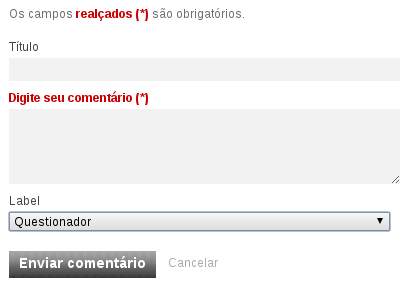
\includegraphics[scale=0.5]{comment-add.png}
\caption{Escolha de etiquetas}
\label{fig:comment-add}
\end{figure}


Todas as pessoas com permissão de visualizar o comentário poderão
visualizar a Etiqueta definida para o comentário
(Figura~\ref{fig:comment-view-label}). A cor definida pela Etiqueta
ajudará aos visualizadores dos comentários a identificar rapidamente o
tipo de comentário.

\begin{figure}[h]
\center
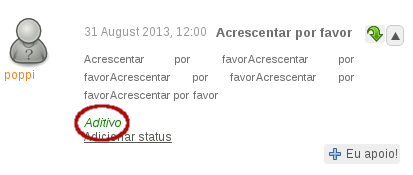
\includegraphics[scale=0.6]{comment-view-label.png}
\caption{Visualização de um comentário com Etiqueta}
\label{fig:comment-view-label}
\end{figure}

\section{Status}

O Status permite a classificação dos comentários por pessoas com
permissões específicas.


\subsection{Definição}

Foi definida uma nova classe {\it Status}
(Apêndice~\ref{App:PluginStatus}) no Plugin de classificação de
comentários para a inclusão da funcionalidade de Classificação por
Status. Os comentários podem ser classificados por vários Status, que possui os
seguintes atributos:
\begin{itemize}
  \item Nome ({\it name}): cada status terá um nome único, que o representará no
ambiente;
  \item Habilitado ({\it enabled}): Os status podem ser habilitados e
desabilitados pelos administradores. Apenas os status habilitados estarão
disponíveis para classificação dos comentários;
  \item Habilita justificativa ({\it enable\_reason}): Os status podem
permitir a inclusão de uma justficativa;
 \item Dono ({\it owner}): Relaciona o status com o usuário que o
definiu. 
\end{itemize}

O sistema registra quando um usuário adiciona um Status a um
comentário. A classe apresentada no
Apêndice~\ref{App:PluginCommentStatusUser} mostra as relações e
validações da relação. Quando um usuário com permissão de moderação de
comentários classifica um comentário é criada a relação no banco de
dados com os seguintes atributos:
\begin{itemize}
  \item Profile ({\it profile}): Referencia o perfil que definiu o
status;
  \item Comment ({\it comment}): Referencia o comentário classificado;
  \item Status ({\it status}): Referencia o status definido;
  \item Reason ({\it reason}): Permite que seja inserida uma
justificativa para o Status escolhido;
\end{itemize}

A definição dessas classes e seus atributos podem ser vistas na
Figura~\ref{fig:status-model}.

\begin{figure}[h]
\center
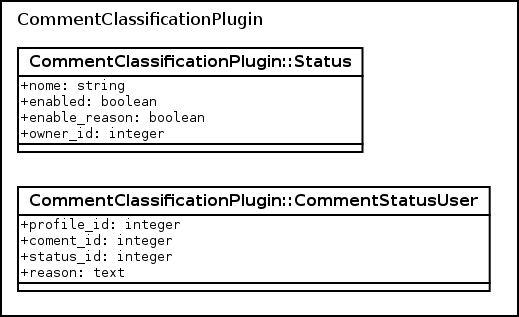
\includegraphics[scale=0.5]{status-model.png}
\caption{Modelagem das classes para definir um status a um comentário}
\label{fig:status-model}
\end{figure}

Os status permitem que pessoas com permissão de moderação de
comentários, os {\it avaliadores}, definam o Status de um comentário e a
justificativa para tal escolha. Cada status definido é registrado no
sistema como um {\it log} de atividades e pode ser visualizado por
pessoas com permissões específicas.

\subsection{Administração}

Para a gestão de {\it Status} dos comentários foi criada uma tela com
a listagem dos status disponíveis no ambiente
(Figura~\ref{fig:plugin-status-admin}). Nessa página o administrador
do ambiente poderá criar, editar e remover qualquer um dos status
listados.

\begin{figure}[h]
\center
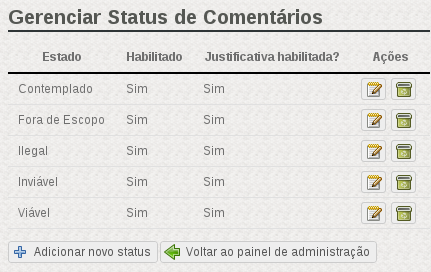
\includegraphics[scale=0.5]{plugin-status-admin.png}
\caption{Tela de gestão dos Status}
\label{fig:plugin-status-admin}
\end{figure}

\begin{figure}[h]
\center
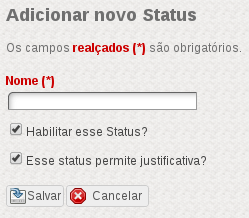
\includegraphics[scale=0.5]{new-status-page.png}
\caption{Criação de status}
\label{fig:new-status-page}
\end{figure}

O formulário de criação de Status pode ser visto na
Figura~\ref{fig:new-status-page}. Nessa página o administrador
do ambiente poderá definir os atributos do status.

\subsection{Utilização}

Na visualização de um comentário do Noosfero foi adicionado um link para
a inclusão de um Status (Figura~\ref{fig:comment-view-status}). Esse
link só será visualizado pelos usuários com permissão de moderação de
comentários.

\begin{figure}[h]
\center
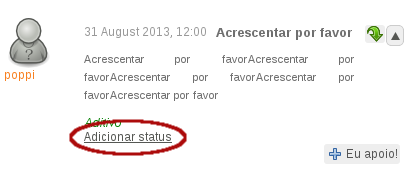
\includegraphics[scale=0.6]{comment-view-status.png}
\caption{Visualização de um comentário com link para adicionar Status}
\label{fig:comment-view-status}
\end{figure}

Cada comentário poderá ter várias justificativas. Cada usuário com
permissão de moderação de comentários poderá incluir várias
justificativas. A ideia é que cada Avaliador leia o histórico de
status e justificativas dos outros Avaliadores e que ocorra uma
discussão até a decisão final sobre o que será feito sobre o trecho
comentado (Figura~\ref{fig:new-status-page-and-history}).

Os status também serão utilizados para ajudar no processo de
consulta e participação popular, então é importante que o histórico e o
debate permitam uma classificação final do Status do comentário. Cada
inclusão de justificativa é registrada no sistema e não pode ser
alterada. Dessa forma é possível saber qual usuário definiu o status,
sua justificativa e a sugestão de novo texto, permitindo uma
auditoria posterior.

\begin{figure}[h]
\center
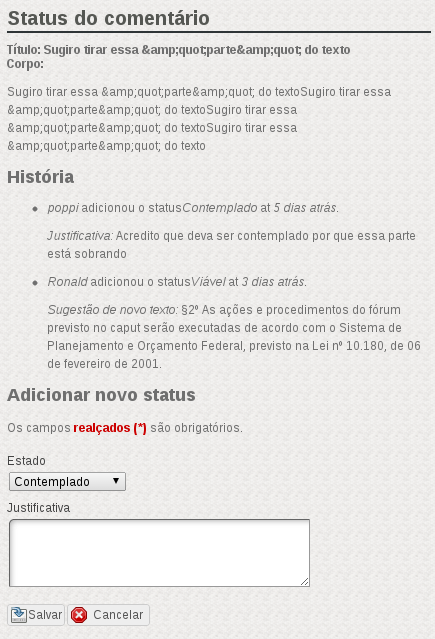
\includegraphics[scale=0.5]{new-status-page-and-history.png}
\caption{Escolha de status}
\label{fig:new-status-page-and-history}
\end{figure}

\section{Apoio}

A funcionalidade Apoio ({\it Support}) permite que usuários concordem com
um comentário.

\subsection{Definição}

Foi definida uma nova classe {\it Support}
(Apêndice~\ref{App:PluginSupport}) no Plugin de classificação de
comentários para a inclusão da funcionalidade de Classificação por
Apoio. O sistema registra quando um usuário apoia um comentário. Quando
um usuário demonstra sua concordância com outro comentário é criada a
relação no banco de dados com os seguintes atributos:
\begin{itemize}
  \item Profile ({\it profile}): Referencia o perfil que definiu apoiou
o comentário;
  \item Comment ({\it comment}): Referencia o comentário classificado;
\end{itemize}

\begin{figure}[h]
\center
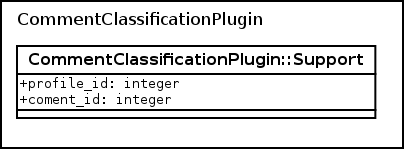
\includegraphics[scale=0.5]{support-model.png}
\caption{Modelagem da classe para apoiar um comentário}
\label{fig:support-model}
\end{figure}

A definição dessa classe e seus atributos podem ser vistas na
Figura~\ref{fig:support-model}.

\subsection{Utilização}

\begin{figure}[h]
\center
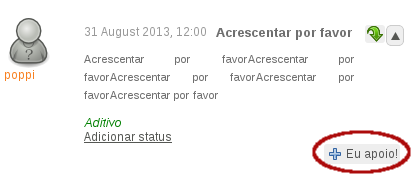
\includegraphics[scale=0.6]{comment-view-support.png}
\caption{Visualização de um comentário com botão para apoiar o
comentário}
\label{fig:comment-view-support}
\end{figure}

Na visualização de um comentário do Noosfero foi adicionado um botão para
que um usuário apoie um comentário
(Figura~\ref{fig:comment-view-support}). Esse botão será visualizado por
todos os usuários com permissão de visualização do comentário.

\section{Personalização por perfil}

As definições realizadas no escopo do ambiente também poderão ser
personalizadas no contexto de um perfil.

Em cada tipo de perfil do Noosfero será possível habilitar e desabilitar
cada uma das classificações {\it Etiqueta}, {\it Status} e {\it Apoio}.
Além disso, também poderá criar novas etiquetas, novos status e
desabilitar etiquetas e status. Um administrador
apenas de perfil não terá permissão para editar nem remover uma etiqueta
ou status do ambiente, podendo apenas desabilitá-los em seu perfil. Por
padrão, todas as etiquetas e status do ambiente são habilitadas no
contexto do perfil.

Em um perfil específico, ao classificar com uma etiqueta ou status, os
usuários terão disponíveis as opções do ambiente e as opções específicas do
perfil.

\section{Estatísticas das classificações}

Todas as classificações do plugin geram estatísticas que podem ser
visualizadas pelos usuários com permissões específicas na tela de
administração do plugin.

\subsection{Label}

Os avaliadores poderão visualizar quantos comentários receberam cada uma
das etiquetas cadastradas no ambiente.

\subsection{Status}

Os avaliadores poderão visualizar quais status foram definidos para
cada um dos comentários, facilitando a conclusão final sobre o que
deverá ser feito sobre o trecho comentado.

\subsection{Support}

Os usuários com permissão de visualização de comentários poderão
visualizar quais e quantos usuários apoiaram determinado comentário.

Os avaliadores poderão visualizar quais comentários foram mais apoiados,
auxiliando o processo de consulta e participação. Os comentários mais
apoiados podem influenciar o status que o avaliador irá definir para um
comentário.

\section{Exportação dos dados}

Os dados resultantes da consulta pública serão exportados no formato CSV
para que possa ser analisado também fora do ambiente. A sugestão de
formatação pode ser visualizada no Apêndice~\ref{App:PluginCSVFile}.

Esse arquivo gerado lista os trechos, seus comentários e as
justificativas e sugestões de alteração de texto de cada um dos
comentários.

\newpage

\section{Considerações finais}

Neste documento foi apresentada a especificação e modelagem do código
desenvolvido para o Portal de Consulta Pública. As telas incluídas nesse
documento é apenas uma sugestão e pode ser alterada após uma avaliação
de um especialista em {\it Design de interfaces} para que seja
assegurada a qualidade visual e de usabilidade do sistema.

Lembramos que para tornar o Portal de Consulta Pública realmente um canal de
consulta e participação popular na discussão e na definição da agenda
prioritária do país, é necessário que além da proposta de código
incluída nesse documento também haja um esforço fora do sistema.

O incentivo à participação nas consultas deve ser feito através de
mobilizações na rede e fora da rede. Essas mobilizações deverão
incentivar a sociedade a registrar suas ideias no Portal de Consulta
Pública, para que assim ela se torne uma das ferramentas de
sistematização das contribuições da sociedade.

\vspace{1cm}

Sem mais nada a acrescentar, coloco-me à disposição.

\vspace{1cm}

\begin{minipage}{\textwidth}
  Brasília/DF, \DiaEntrega \ de \MesEntrega\\[1cm]
  \textbf{\MyName}\\
  \small Consultora do PNUD
\end{minipage}

\newpage
\appendix
\appendixpage
\section{Foo bar}
\label{foobar}

%\lstinputlisting{observatorio.rb}


\end{document}
